\documentclass[a4paper,11pt]{report}

\usepackage[utf8]{inputenc}
\usepackage[T1]{fontenc}
\usepackage[english]{babel}
\usepackage{amsfonts}
\usepackage{amsmath}
\usepackage{amsthm}
\usepackage[pdftex]{graphicx}
\usepackage{float}
\usepackage{listings}
\usepackage{fullpage}
%
\newcommand{\alinea}{
\hspace*{0.5cm}}
%
\renewcommand{\thesection}{\arabic{section}}
%
\newtheorem{definition}{Definition}
\newtheorem{law}{S.E. law}
%
\title{Basic Principles of Software Evolution: Summary}
\author{Anthony Rouneau}
%
\begin{document}
\maketitle
\newpage
%
\section{Technical aspects of Software Evolution}
	Here are some technical aspects of the
		Software Evolution.
	%
	\begin{itemize}
		\setlength{\itemsep}{0pt}		
		\setlength{\parskip}{0pt}		
		\setlength{\parsep}{0pt}	
		\item Version management
		\item Software quality measurement
			and improvement
		\item Legacy systems and migration
		\item Reverse Engineering and program
			comprehension
		\item Model-driven evolution
		\item Change propagation and program
			comprehension
		\item Traceability
		\item Co-evolution
		\item Consistency maintenance
		\item Regression testing
		\item Design for change
		\item Visualisation and statistical
			analysis of evolution histories
		\item Software product lines and 
			product families
	\end{itemize}
	%
	\begin{definition}
		\textbf{Reverse engineering} --
			Process of analysing a project to fully
			understand it and to extract the key
			issues. Mostly, the system is a 
			large legacy system with a poor
			 documentation and in a bad shape.
			 Visualisation techniques can help.
	\end{definition}
	%
	\begin{definition}
		\textbf{Re-engineering} -- 
			Horseshoe process (cf. figure
			\ref{fig:reengineering}) that targets
			to rethink a project in order to
			address one or multiple problems.
	\end{definition}
	%
	\begin{figure}[H]
		\centering
		\includegraphics[scale=0.2]{figures/%
		reengineering}
		\caption{Re-engineering}%
		\label{fig:reengineering}
	\end{figure}\noindent
	%
	\subsection{Visualisation techniques}
		Visualisation techniques are useful to
			\textbf{understand} the way a
			software works, but also to understand
			the \textbf{complexity} of a software.
			There is five types of visualisation.
		%
		\subparagraph{Code duplication}
			The duplication of the code can be 
			visualised as a dotplot, showing 
			the similarity between multiple
			files. \textit{CCFinderX, Duploc}
		%			
		\subparagraph{Dependencies}
			The dependencies between the class
			or with external libraries can
			be shown of graphs, binding 
			two dependant classes. \textit{Stan, 
			IntelliJ IDEA, ...}
		%
		\subparagraph{Metrics}
			The quality metrics can be 
			visualised on multiple sort of
			views, 2D, 3D, ... \textit{3D Treemap,
			Sunburst, ...}
		%
		\subparagraph{Change}
			The change of the software over time
			can be visualised, comparing the 
			different versions. \textit{Chronia}.	
		%
		\subparagraph{Quality}
			The metrics can be summarized into 
			one quality metrics that can be visualised.
			The managerial evolution can be observed
			over time. The complexity can be 
			viewed to ease reverse engineering.
			\textit{Code Crawler, X-Ray, ...}
			\begin{itemize}
				\setlength{\itemsep}{0pt}		
				\setlength{\parskip}{0pt}		
				\setlength{\parsep}{0pt}	
				\item \textbf{Coarse-Grained
					visualisation} -- 	Multiple
					metrics visible in one view.
					Can be used to reverse engineer.
				\item \textbf{Fine-Grained 
					visualisation} -- Class 
					Blueprint views can be used
					to understand classes 
					and class hierarchies, using
					a pattern language.
				\item \textbf{Evolution Matrix} --
					Using a pattern language,
					one can analyse the system 
					evolution and/or the classes
					evolution.
			\end{itemize}
		%
	%
%
\section{Managerial aspects}
	\begin{itemize}
		\item Traditional process model
		\item Evolutionary process model
			\begin{itemize}	
				\setlength{\itemsep}{0pt}		
				\setlength{\parskip}{0pt}		
				\setlength{\parsep}{0pt}	
				\item Staged life-cycle
				\item Iterative and incremental 
					process
				\item Agile methods
			\end{itemize}
		\item Software configuration management
			\begin{itemize}
				\setlength{\itemsep}{0pt}		
				\setlength{\parskip}{0pt}		
				\setlength{\parsep}{0pt}	
				\item Change management
				\item Version management
			\end{itemize}
		\item Estimation techniques
			\begin{itemize}	
				\setlength{\itemsep}{0pt}		
				\setlength{\parskip}{0pt}		
				\setlength{\parsep}{0pt}	
				\item Change impact analysis
				\item Effort estimation
				\item Cost estimation
				\item Change metrics
			\end{itemize}
	\end{itemize}
	%
	\subsection{Evolution process}
		The evolution of a software follows steps,
			defined in the chosen process model.
			The \textbf{urgent changes} can bypass 
			such model to be available faster.
		\begin{figure}[H]
			\centering
			\includegraphics[scale=0.75]{figures/%
				waterfall.png}
			\caption{Traditional waterfall process model}
		\end{figure}\noindent
		%
		\begin{figure}[H]
			\centering
			\includegraphics[scale=0.75]{figures/%
				evolutionary.png}
			\caption{Evolutionary process}
		\end{figure}\noindent
		%
		\begin{minipage}{0.5\textwidth}
			\begin{figure}[H]
				\hspace*{-1cm}
				\includegraphics[scale=0.7]{figures/%
					evolution_spiral.png}
				\caption{Evolution spiral model}
			\end{figure}\noindent
		\end{minipage}\hfill
		\begin{minipage}{0.475\textwidth}
			\vspace*{1cm}
			\begin{figure}[H]
				\centering
				\includegraphics[scale=0.575]{figures/%
					evolution_staged_life.png}
				\caption{Evolution staged life model}
			\end{figure}\noindent
		\end{minipage}
		%
	%
	\subsection{Software configuration management}
		\noindent
		Changing a part of the software may
			affect other parts. Software
			configuration management consists 
			of predicting the total number
			of changes required by an evolution and
			making the software the less 
			subject to change by reducing
			coupling and dependences.
		%
		\begin{definition}
			\textbf{Ripple effect} -- 
				The phenomenon where a change 
				in one piece of a software system
				affects at least one other area of 
				the same software system (either
				directly or indirectly).
		\end{definition}
		%
		\begin{definition}
			\textbf{Change propagation} --
				Occurs when making a change to one 
				part of a software system
				requires other system parts that 
				depend on it to be changed as well.
				These dependent system parts can on 
				their turn require changes in
				other system parts. In this way, a 
				single change to one system part
				may lead to a propagation of changes 
				to be made throughout the
				entire software system.
		\end{definition}
		%
		When a component is changed, visit every
			module that includes the component
			and check if it still fits.
			If a change is required, the same process
			is applied, taking the module as
			component.
		%
	%
%
\newpage
%
\section{Software Maintenance}\noindent
	The software maintenance is used
		to avoid \textbf{large} software to become 
		legacy systems. In fact, adding
		new functionalities without 
		considering code quality gives rise
		to \textbf{technical debt}.
	\begin{definition}
		\textbf{Technical debt} -- 
			Lack of quality in the code due to 
			modifications done in a hurry.
			The project is unclean while the debt
			has not been paid back through 
			re-engineering. Measured in days; 
			an estimation of time that would take
			to accomplish the pending tasks.
	\end{definition}
	%
	\begin{definition}
		\textbf{Software maintenance (1)} -- 
			The process of modifying a software 
			system or component after delivery 
			to correct faults, improve 
			performance or other attributes, 
			or adapt to a changed environment
	\end{definition}
	%
	\begin{definition}
		\textbf{Software maintenance (2)} -- 
			The software product undergoes 
			modification to code and associated 
			documentation due to a problem or
			the need for improvement. 
			The objective is to modify
			the existing software product 
			while preserving its integrity
	\end{definition}\noindent
	%
	The software change is :
	\begin{itemize}
		\setlength{\itemsep}{0pt}		
		\setlength{\parskip}{0pt}		
		\setlength{\parsep}{0pt}	
		\item \textbf{Unpredictable} --
			All the changes and bugs can not be
			anticipated in the design.
		\item \textbf{Expensive} --
			You generally don't get paid to solve bugs but
			to develop as fast as possible.
		\item \textbf{Difficult}-- The errors are hard
			to find and the source code can be messy.
	\end{itemize}
	%
	\subsection{Legacy system}
		Characteristics : 
		\begin{itemize}
			\setlength{\itemsep}{0pt}		
			\setlength{\parskip}{0pt}		
			\setlength{\parsep}{0pt}	
			\item Original developers no longer
				available
			\item Outdated development methods
				used
			\item Extensive patches and modifications 
				have been made
			\item Missing or outdated documentation
		\end{itemize}
	%
	\subsection{Parnas' ageing software}
		Symptoms :
		\begin{itemize}
			\item Lack of knowledge
				\begin{itemize}
					\setlength{\itemsep}{0pt}		
					\setlength{\parskip}{0pt}		
					\setlength{\parsep}{0pt}	
					\item Insufficient, inconsistent or
						obsolete documentation
					\item Departure of original 
						developers
					\item Disappearance of inside 
						knowledge about the system
					\item Missing tests
				\end{itemize}
			\item Code symptoms
				\begin{itemize}
					\setlength{\itemsep}{0pt}		
					\setlength{\parskip}{0pt}		
					\setlength{\parsep}{0pt}	
					\item Duplicated code, code smells, 
						lack of modularity
					\item Lack of overall structure 
						or architecture
				\end{itemize}
			\item Process symptoms
				\begin{itemize}	
					\setlength{\itemsep}{0pt}		
					\setlength{\parskip}{0pt}		
					\setlength{\parsep}{0pt}	
					\item Constant need for bug fixes
						Too long time to fix bugs or to 
						add new functionality
					\item Difficult to separate
						functionalities
				\end{itemize}
		\end{itemize}
		%
	%
	\newpage
	%
	\subsection{Necessity of software change}
		Software change is inevitable because:
		%
		\begin{itemize}
			\setlength{\itemsep}{0pt}		
			\setlength{\parskip}{0pt}		
			\setlength{\parsep}{0pt}	
			\item New requirements emerge when the 
				software is used or developed.
			\item The business environment changes.
				\begin{itemize}	
					\setlength{\itemsep}{0pt}		
					\setlength{\parskip}{0pt}		
					\setlength{\parsep}{0pt}	
					\item New customers
					\item New demands
					\item Organisational changes
					\item Competitors
				\end{itemize}
			\item Errors must be repaired
				\begin{itemize}
					\setlength{\itemsep}{0pt}		
					\setlength{\parskip}{0pt}		
					\setlength{\parsep}{0pt}	
					\item Bug fix routine
					\item Emergency fix
				\end{itemize}
			\item Hardware changed
			\item Improvements needed in efficiency
			\item New technologies have to be used
			\item Changes in data formats
				\begin{itemize}
					\setlength{\itemsep}{0pt}		
					\setlength{\parskip}{0pt}		
					\setlength{\parsep}{0pt}	
					\item New standards
					\item New currency, ...
				\end{itemize}
		\end{itemize}
		%
	%
	\subsection{Types of software maintenance}
		\begin{itemize}
			\setlength{\itemsep}{0pt}		
			\setlength{\parskip}{0pt}		
			\setlength{\parsep}{0pt}	
			\item \textbf{Adaptive} -- 
				Adapt a software after delivery 
				to support new technologies
			\item \textbf{Corrective} -- 
				Repair errors discovered after delivery
			\item \textbf{Perfective} -- 
				Add new functionalities to the 
				software or improve it after delivery\\
				\alinea\alinea\alinea
				\alinea
				\alinea$\Longrightarrow$ \textit{main reason}
			\item \textbf{Preventive} --
				Correct latent faults before they
				become effective ones.
		\end{itemize}
		%
		\begin{center}
			\begin{tabular}{|c|c|c|}
				\hline
				\textit{When? / Why?} & 
					\textbf{Correction} &
					\textbf{Enhancement}\\
				\hline
				\textbf{Proactive} (before it happens) & 
					Preventive & Perfective\\
				\hline		
				\textbf{Reactive} (after it happened) & 
					Corrective & Adaptive\\			
				\hline
			\end{tabular}
		\end{center}
		%
		\begin{figure}[H]
			\centering
			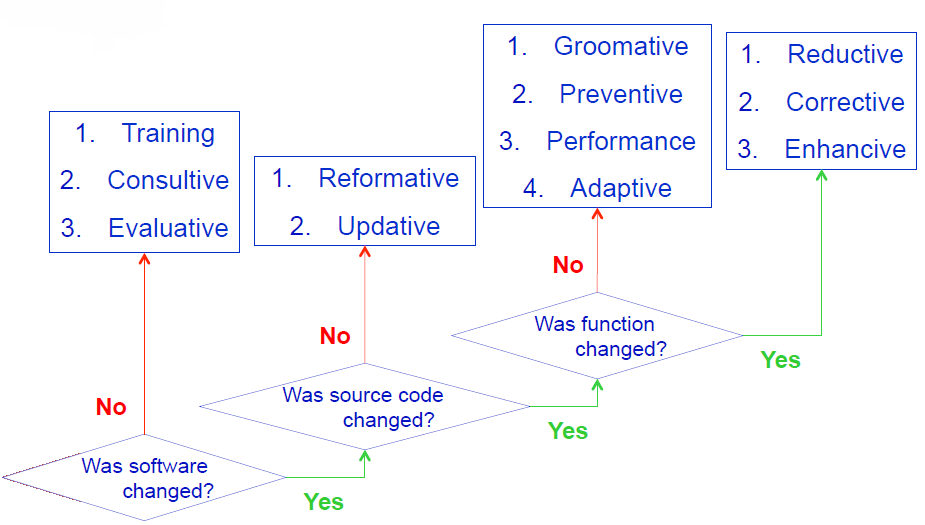
\includegraphics[scale=0.6]{figures/types.PNG}
		\end{figure}\noindent
		%
	%
	\subsection{Seven deadly sins}\noindent
		According to SonarQube, there are seven
			deadly technical debt that should be 
			avoid as much as possible.	
		\begin{itemize}
			\setlength{\itemsep}{0pt}		
			\setlength{\parskip}{0pt}		
			\setlength{\parsep}{0pt}	
			\item Bugs and Potential Bugs
			\item Coding Standards Breach
			\item Duplications
			\item Lack of Unit Tests
			\item Bad Distribution of Complexity
			\item Spaghetti Design
				\begin{itemize}	
					\setlength{\itemsep}{0pt}		
					\setlength{\parskip}{0pt}		
					\setlength{\parsep}{0pt}	
					\item Cyclic dependencies
					\item High coupling
					\item Low cohesion
				\end{itemize}
			\item Not Enough or Too Many Comments
		\end{itemize}
	%
	\subsection{Clones}\noindent
		There are three types of clones
		\begin{itemize}
			\setlength{\itemsep}{0pt}		
			\setlength{\parskip}{0pt}		
			\setlength{\parsep}{0pt}	
			\item \textbf{Type 1} -- Same code,
				except for the line breaks, etc...
			\item \textbf{Type 2} -- Same code,
				except for the variable/method
				names.
			\item \textbf{Type 3} -- Same code 
				modulo some changes/additions.
		\end{itemize}
	%
%
\end{document}
